\chapter{The Elliptic Genus of K3 and \texorpdfstring{$N=4$}{N = 4} Characters}\label{ch:ellgenus}

How much of a quantum theory can be computed exactly? For a supersymmetric theory the
answer is ``more than one would expect'', because a partition function with the sign
$(-1)^F$ inserted, $F$ the fermion number, counts states with signs that cancel in pairs.
What survives the cancellation is a robust quantity: it does not change when the couplings
change, and it can be evaluated in whatever limit is convenient. The simplest such quantity
is the Witten index. This chapter is about its refinement for a two-dimensional
conformal field theory, the \emph{elliptic genus}, evaluated for the sigma model whose
target space is the K3 surface of \cref{ch:k3}. The result is remarkably rigid: the elliptic
genus of K3 is a weak Jacobi form of weight $0$ and index $1$, a space of functions that is
one-dimensional, so the whole function is determined by a single number, the Euler number
$24$. Rigid does not mean empty. When the same function is expanded in characters of the
$N=4$ superconformal algebra at central charge $c=6$, the symmetry algebra of any K3 sigma
model, the multiplicities are $20$, $-2$ and then $2A_n$ with
\begin{equation}\label{eq:ellgenus:An}
 A_1,A_2,A_3,A_4,A_5,\dots \;=\;45,\;231,\;770,\;2277,\;5796,\;\dots
\end{equation}
The first five of these are dimensions of irreducible representations of the sporadic
Mathieu group $\Mtf$, an observation of Eguchi, Ooguri and Tachikawa
\source{EOT §1, ll.~197--233} that opens the ``Mathieu moonshine''\index{Mathieu moonshine} story of
\cref{ch:m24,ch:moonshine}. Before we can appreciate the observation we need to know
precisely what is being counted, and that is the purpose of this chapter. The chapter
answers three questions. What is an elliptic genus and why is it independent of the moduli
of K3? Why is it fixed by the number $24$? And what are the $N=4$ characters in which it
is expanded, and how are the numbers in \eqref{eq:ellgenus:An} extracted?

Throughout, $q=\ee^{2\pi\ii\tau}$ with $\tau$ in the upper half-plane and $y=\ee^{2\pi\ii z}$
with $z\in\C$. We use the conventions of \cref{ch:cft} for the Virasoro algebra, $L_0$,
central charge $c$, and the $q^{L_0-c/24}$ form of a partition function.

\section{Counting with a sign}\label{sec:ellgenus:index}

\subsection{The Witten index}

Consider a quantum theory with a Hamiltonian $H$, a fermion-number operator $(-1)^F$ that
commutes with $H$, and a supercharge $Q$ with
\begin{equation}\label{eq:ellgenus:susy}
 Q^2 = H,\qquad (-1)^F Q = -Q\,(-1)^F .
\end{equation}
\index{Witten index}
The second relation says that $Q$ maps bosons ($(-1)^F=+1$) to fermions and back. The
\emph{Witten index} is
\begin{equation}\label{eq:ellgenus:witten}
 I \;=\; \Tr\,(-1)^F \ee^{-\beta H}.
\end{equation}
The trace is over the whole Hilbert space, but almost everything cancels. Take an
eigenstate $\ket{\psi}$ of $H$ with eigenvalue $E>0$. Then $Q\ket{\psi}$ is a nonzero state
(because $\bra{\psi}Q^2\ket{\psi}=E\ne0$) with the same energy and the opposite sign of
$(-1)^F$. So the states of positive energy come in boson--fermion pairs, and each pair
contributes $(+1-1)\ee^{-\beta E}=0$ to \eqref{eq:ellgenus:witten}. Only the states with
$E=0$, which are annihilated by $Q$ and need not be paired, contribute, and they contribute
$\pm1$ independently of $\beta$:
\begin{equation}\label{eq:ellgenus:index_count}
 I \;=\; n_B^{(E=0)} - n_F^{(E=0)} .
\end{equation}
This has two consequences. First, $I$ is an integer. Second, if a parameter of the theory is
varied continuously, states can leave or reach $E=0$ only in boson--fermion pairs, so $I$
does not change. \emph{The index is a topological invariant of the theory.}

\begin{physicsbox}[Why a sign makes a quantity computable]
An ordinary partition function $\Tr\,\ee^{-\beta H}$ knows every energy level and is as hard
to compute as the theory itself. Inserting $(-1)^F$ makes the excited states invisible, and
what is left can be computed at any convenient value of the parameters: at large volume, where
the sigma model is classical geometry, or at a special symmetric point, where it is a
solvable conformal field theory. The elliptic genus keeps this property while retaining much
more information than a single integer, because it inserts $(-1)^F$ only for one chirality
and keeps track of the other quantum numbers by fugacities.
\end{physicsbox}

\subsection{The refinement: one chirality at a time}

Now let the theory be a two-dimensional conformal field theory with $N=2$ superconformal
symmetry in both the left- and the right-moving sector (a ``$(2,2)$ theory''). Each sector
has its own Virasoro generators $L_n$, $\bar L_n$, its own $U(1)_R$ current with zero mode
$J_0$, $\bar J_0$, and its own fermion number. The theory is placed on a torus with modular
parameter $\tau$, in the sector in which the fermions are periodic in both directions on the
spatial circle (the Ramond--Ramond, or RR, sector). Following
\source{GHV §2, eq.~(2.1), ll.~104--113}, the \emph{elliptic genus} is
\index{elliptic genus}
\begin{equation}\label{eq:ellgenus:def}
 \phi(\tau,z) \;=\; \Tr_{\mathcal H_{RR}}\Big(
   q^{L_0-\frac c{24}}\,\ee^{2\pi\ii zJ_0}\,(-1)^F\;
   \bar q^{\bar L_0-\frac{\bar c}{24}}\,(-1)^{\bar F}\Big).
\end{equation}
Compare with \eqref{eq:ellgenus:witten}: in a conformal field theory on a circle the
Hamiltonian is $L_0+\bar L_0-\frac{c+\bar c}{24}$, and $\ee^{-\beta H}$ has become
$q^{L_0-c/24}\bar q^{\bar L_0-\bar c/24}$. The novelty is the factor $\ee^{2\pi\ii zJ_0}$,
which keeps track of the left-moving $U(1)_R$ charge, and the fact that
$q^{L_0-c/24}$ is not accompanied by a compensating right-moving quantity: the pairing
argument is applied to the right-moving supercharge $\bar G_0$ only. In the Ramond sector
$\bar G_0^2=\bar L_0-\bar c/24$, and $\bar G_0$ commutes with $L_0$, $J_0$ and $(-1)^F$. The
argument of the previous subsection, applied to $\bar G_0$, therefore shows that only states
with $\bar L_0=\bar c/24$ (\emph{right-moving Ramond ground states}\index{Ramond ground states}) contribute, so
\eqref{eq:ellgenus:def} is independent of $\bar q$: it is a holomorphic function of $\tau$
\source{GHV §2, ll.~115--118}. On the left-moving side no cancellation is forced, and the
elliptic genus is a genuine $q$-series
\begin{equation}\label{eq:ellgenus:fourier}
 \phi(\tau,z)=\sum_{n\ge0,\;\ell\in\Z} c(n,\ell)\,q^n y^\ell ,
\end{equation}
whose coefficients count, with sign, right-moving ground states of left-moving level $n$ and
left charge $\ell$ \source{GHV §2, eq.~(2.4), ll.~145--153}.

Three specializations are worth memorizing. Setting $z=0$ removes the charge grading and
leaves $\Tr(-1)^{F+\bar F}q^{L_0-c/24}$ in which now the left-moving pairing also operates,
so only the $q^0$ term survives:
\begin{equation}\label{eq:ellgenus:z0}
 \phi(\tau,0) \;=\; \text{Witten index of the RR sector} \;=\; \chi(M)
\end{equation}
for a sigma model with target $M$, because the RR ground states are in one-to-one
correspondence with the cohomology of $M$ and the sign $(-1)^{F+\bar F}$ is $(-1)^{p+q}$ on
$H^{p,q}(M)$. Setting $z=\tfrac12$ (so $y=-1$) weights the charges by $(-1)^\ell$, and the
$q^0$ term becomes $\sum(-1)^{p+q}(-1)^{p-1}h^{p,q}=-\sum_q(-1)^q\sum_p h^{p,q}$, which for a
surface is minus the Hirzebruch signature $\sigma(M)=\sum_{p,q}(-1)^qh^{p,q}$; for K3, with
$b^+=3$ and $b^-=19$ (\cref{ch:k3lattice}), $\sigma=-16$ and the $q^0$ term is $+16$.
Finally the $q^0$ term at
general $y$ is the $\chi_y$ genus\index{chi_y genus@$\chi_y$ genus} $\sum_{p,q}(-1)^{p+q}h^{p,q}y^{p-c/6}$; the shift by $c/6$ is
the charge of the Ramond ground state of lowest $J_0$ and will be explained in
\cref{sec:ellgenus:n4}. \source{EOT §1, ll.~74--77} record the K3 values: $\phi(\tau,0)=24$
and $\phi(\tau,\tfrac12)=16+O(q)$, the Euler number and the signature of K3 from \cref{ch:k3}.

\section{The K3 sigma model and its \texorpdfstring{$N=4$}{N = 4} algebra}\label{sec:ellgenus:n4}

\subsection{Central charge}

The sigma model with target K3 has four real bosonic fields (the coordinates of the
four-real-dimensional surface) and, in the supersymmetric model, four real fermionic
partners of each chirality. A free boson contributes $c=1$ and a free Majorana fermion
$c=\tfrac12$ to the central charge (\cref{ch:cft}), so
\begin{equation}\label{eq:ellgenus:c6}
 c=\bar c=4\cdot1+4\cdot\tfrac12=6 .
\end{equation}
\index{central charge!of the K3 sigma model}
The sigma model on K3 is of course not free: the metric is curved. But the central charge is
protected. A Ricci-flat target gives a conformal theory (\cref{ch:backgrounds}), and $c$ can
be read off at large volume, where the curvature is negligible and the theory is a free
theory of $4+4$ fields locally. The number $6$ is what enters the index of the Jacobi form
below, and it is the number the Lean declaration \lean{central\_charge\_k3\_eq\_six} records
(\cref{sec:ellgenus:lean}).

\subsection{From \texorpdfstring{$N=2$}{N = 2} to \texorpdfstring{$N=4$}{N = 4}}

A Kähler target gives an $N=2$ superconformal algebra on each side: the stress tensor $T$,
two supercurrents $G^\pm$ of charge $\pm1$, and a $U(1)_R$ current $J$. Unitary
representations obey the bound
\begin{equation}\label{eq:ellgenus:bps}
 h\;\ge\;\frac{|q|}{2}
\end{equation}
between the conformal weight $h$ and the $U(1)$ charge $q$ of a primary state in the NS
sector (standard; not checked against a source in this book's library), and the states that
saturate it with $q\ge0$ are the \emph{chiral primaries}. Under the identification of the
sigma model with geometry, chiral primaries of charge $q=p$ correspond to the holomorphic
$p$-forms, $H^{p,0}(M)$. For K3, $h^{0,0}=h^{2,0}=1$ and $h^{1,0}=0$ (\cref{ch:k3}), so there
are exactly two: the identity and the state $\Omega$ of charge $2$ and weight $1$, created by
the holomorphic two-form. This count, $1+0+1=2$, is the content of the Lean declaration
\lean{k3\_chiral\_primary\_total} (\cref{sec:ellgenus:lean}).
\index{chiral primary}

The existence of $\Omega$ with $h=1$, $q=2$, together with its conjugate, is exactly what
enlarges the symmetry. A hyperk\"ahler target has not one but a two-sphere of complex
structures, and the sigma model has an $SU(2)$ of $R$-currents of which $J$ is the Cartan
generator; the two extra currents are the spectral-flow images of the identity, of weight $1$
and charge $\pm2$. The resulting algebra is the \emph{$N=4$ superconformal algebra}
\index{N=4 superconformal algebra@$N=4$ superconformal algebra} with four supercurrents and an
affine $SU(2)$ at level $k=c/6=1$ \source{EOT §1, ll.~43--53}. Its unitary representations
are labelled by $h$ and by the $SU(2)$ spin $\ell$ of the highest-weight state; at level
$k=1$ the possible spins are $\ell=0,\tfrac12$. The $U(1)$ charge of the $N=2$ subalgebra is
$J_0=2J_0^3$, which is why \source{EOT §1, eq.~(1.1), ll.~43--46} write the fugacity as
$\ee^{4\pi\ii zJ^3_0}$ where \eqref{eq:ellgenus:def} has $\ee^{2\pi\ii zJ_0}$; the two are the
same operator.

\subsection{Ramond ground states and spectral flow}

In the Ramond sector the supercharge $G_0$ satisfies $G_0^2=L_0-c/24$, so Ramond ground
states have $h=c/24=\tfrac14$. The NS and R sectors are related by \emph{spectral flow}\index{spectral flow},
the one-parameter family of automorphisms
\begin{equation}\label{eq:ellgenus:flow}
 L_0\;\mapsto\;L_0+\eta J_0+\eta^2\frac c6,\qquad J_0\;\mapsto\;J_0+\eta\frac c3
\end{equation}
\source{GHV §2, eq.~(2.7), ll.~168--187}; $\eta=\pm\tfrac12$ maps NS to R. Flow the NS
vacuum ($h=0$, $q=0$) by $\eta=-\tfrac12$: it acquires $h=\tfrac14\cdot\tfrac c6=\tfrac14$ and
$J_0=-\tfrac c6=-1$, a Ramond ground state of charge $-1$. Flow $\Omega$ ($h=1$, $q=2$) the
same way: $h=1-1+\tfrac14=\tfrac14$, $J_0=2-1=1$. The chiral primaries of charge $p$ become
Ramond ground states of charge $p-c/6=p-1$, which explains the shift in the $\chi_y$ genus
stated after \eqref{eq:ellgenus:z0}. The $24$ RR ground states of K3 are graded by left
charge as
\begin{equation}\label{eq:ellgenus:q0}
 \phi_{K3}(\tau,z)\big|_{q^0}\;=\;2y^{-1}+20+2y ,
\end{equation}
two states each of charge $\mp1$ (from $h^{0,0}+h^{0,2}$ and $h^{2,0}+h^{2,2}$, all with sign
$+$) and twenty of charge $0$ (from $h^{1,1}=20$, sign $(-1)^{1+1}=+$; $h^{1,0}=h^{1,2}=0$
would have contributed with a minus sign). We will recover \eqref{eq:ellgenus:q0} from the
theta-function formula in a moment.

\section{The elliptic genus as a weak Jacobi form}\label{sec:ellgenus:jacobi}

\subsection{Jacobi forms}

The elliptic genus is a torus partition function, so modular transformations of $\tau$ act
on it; and spectral flow by an integer amount, $z\mapsto z+\ell\tau+\ell'$, is a symmetry of
the spectrum. Together with unitarity these facts imply \source{GHV §2, ll.~118--122} that
$\phi$ is a \emph{weak Jacobi form} of weight $w=0$ and index
\begin{equation}\label{eq:ellgenus:index}
 m\;=\;\frac c6 ,
\end{equation}
\index{Jacobi form!weak}
i.e.\ a holomorphic function on $\mathbb H\times\C$ satisfying
\begin{align}
 \phi\Big(\frac{a\tau+b}{c\tau+d},\frac z{c\tau+d}\Big)
   &= (c\tau+d)^w\,\ee^{2\pi\ii m\frac{cz^2}{c\tau+d}}\,\phi(\tau,z),
   \qquad \begin{pmatrix}a&b\\c&d\end{pmatrix}\in\SLZ,\label{eq:ellgenus:jac1}\\
 \phi(\tau,z+\ell\tau+\ell')&=\ee^{-2\pi\ii m(\ell^2\tau+2\ell z)}\,\phi(\tau,z),
   \qquad \ell,\ell'\in\Z,\label{eq:ellgenus:jac2}
\end{align}
with a Fourier expansion \eqref{eq:ellgenus:fourier} in which $n\ge0$ (``weak'') and
$c(n,\ell)=(-1)^wc(n,-\ell)$ \source{GHV §2, eqs.~(2.2)--(2.4), ll.~122--153}. (In
\eqref{eq:ellgenus:jac1} the letter $c$ is a matrix entry, not the central charge.) Where does
the index come from? Apply \eqref{eq:ellgenus:jac2} with $\ell=1$, $\ell'=0$ to a single term
$q^ny^{\ell_0}$ of the expansion: $y\mapsto qy$ turns it into $q^{n+\ell_0}y^{\ell_0}$, and the
prefactor $\ee^{-2\pi\ii m(\tau+2z)}=q^{-m}y^{-2m}$. So the coefficient of $q^{n}y^{\ell_0}$
must equal the coefficient of $q^{n+\ell_0+m}y^{\ell_0+2m}$; with $m=c/6$ this is precisely
the statement that the spectrum is invariant under the spectral flow
\eqref{eq:ellgenus:flow} with $\eta=1$. Iterating, one finds that $c(n,\ell)$ depends on
$(n,\ell)$ only through the discriminant $4mn-\ell^2$ and $\ell \bmod 2m$. For $m=1$ the
second datum is redundant and
\begin{equation}\label{eq:ellgenus:disc}
 c(n,\ell)\;=\;C(4n-\ell^2)\qquad\text{for a weak Jacobi form of index }1.
\end{equation}
We will see this structure explicitly in \cref{tab:ellgenus:coeffs}.

For K3, $m=1$. The crucial fact, quoted in \source{EOT §1, ll.~69--73} and standard in the
theory of Jacobi forms, is that the space of weak Jacobi forms of weight $0$ and index $1$ is
one-dimensional \TL. Its generator is usually called $\phi_{0,1}$, normalized by
$\phi_{0,1}(\tau,0)=12$. Since $\phi_{K3}(\tau,0)=\chi(K3)=24$,
\begin{equation}\label{eq:ellgenus:phi01}
 \phi_{K3}\;=\;2\,\phi_{0,1}.
\end{equation}
This is the sense in which the elliptic genus of K3 is fixed by the single number $24$: any
sigma model on any K3 surface, at any point of the moduli space of \cref{ch:stringsk3}, has
the same elliptic genus. \source{GHV §2, eq.~(2.6), ll.~161--167} work with the rescaled
$\phi_{1A}=\tfrac12\phi_{K3}=\phi_{0,1}$; we keep EOT's normalization $\phi_{K3}$ and will
return to the factor $2$ in \cref{sec:ellgenus:2An}.

\subsection{Theta functions and the formula for K3}

We use the Jacobi theta functions in the product form of \source{GHV App.~A, eq.~(A.1),
ll.~1453--1490}, together with the Dedekind function $\eta$:
\begin{align}
 \eta(\tau)&=q^{1/24}\prod_{n\ge1}(1-q^n),\label{eq:ellgenus:eta}\\
 \vartheta_1(\tau,z)&=-\ii\,q^{1/8}y^{1/2}\prod_{n\ge1}(1-q^n)(1-yq^n)(1-y^{-1}q^{n-1}),
   \label{eq:ellgenus:th1}\\
 \vartheta_2(\tau,z)&=q^{1/8}\,(y^{1/2}+y^{-1/2})\prod_{n\ge1}(1-q^n)(1+yq^n)(1+y^{-1}q^n),
   \label{eq:ellgenus:th2}\\
 \vartheta_3(\tau,z)&=\prod_{n\ge1}(1-q^n)(1+yq^{n-1/2})(1+y^{-1}q^{n-1/2}),\label{eq:ellgenus:th3}\\
 \vartheta_4(\tau,z)&=\prod_{n\ge1}(1-q^n)(1-yq^{n-1/2})(1-y^{-1}q^{n-1/2}).\label{eq:ellgenus:th4}
\end{align}
\index{theta functions}
(In \eqref{eq:ellgenus:th2} we have written $2\cos\pi z=y^{1/2}+y^{-1/2}$.) Each is the
partition function of a single complex fermion with a specified spin structure on the torus:
$\vartheta_1$ is the RR-sector trace with $(-1)^F$ inserted, which is why it vanishes at $z=0$
where the two fermion zero modes give $y^{1/2}-y^{-1/2}\to0$; $\vartheta_2$ is the R-sector
trace without the sign; $\vartheta_3,\vartheta_4$ are the NS-sector traces without and with
the sign. The elliptic genus of K3 was computed by Eguchi, Ooguri, Taormina and Yang
(reference~[2] of EOT, ll.~1013--1014), and reads \source{EOT §1, eq.~(1.2), ll.~56--68}
\begin{equation}\label{eq:ellgenus:ZK3}
 \phi_{K3}(\tau,z)\;=\;8\left[\Big(\frac{\vartheta_2(\tau,z)}{\vartheta_2(\tau,0)}\Big)^2
   +\Big(\frac{\vartheta_3(\tau,z)}{\vartheta_3(\tau,0)}\Big)^2
   +\Big(\frac{\vartheta_4(\tau,z)}{\vartheta_4(\tau,0)}\Big)^2\right].
\end{equation}
The structure is transparent at the orbifold point $T^4/\Z_2$ of \cref{ch:kummer}: the three
terms are the three nontrivial sectors of the $\Z_2$ orbifold (untwisted with the $\Z_2$
inserted, twisted, and twisted with the $\Z_2$ inserted), each a ratio of fermion to boson
determinants, and $8$ is the normalization forced by the Witten index. The untwisted
sector without insertion is the elliptic genus of $T^4$, which vanishes because of the
fermion zero modes. (This orbifold reading is standard; it is not checked against a source
in this book's library, and we use it only as motivation.) Since \eqref{eq:ellgenus:ZK3} is a weak Jacobi form of weight $0$ and
index $1$ (each ratio is: the theta functions all have index $\tfrac12$ and weight
$\tfrac12$, and the three are permuted by $\SLZ$), and since the space is one-dimensional, the
formula is correct for every K3 sigma model once it is correct for the orbifold.

\subsection{Worked example: the first coefficients}\label{sec:ellgenus:worked1}

Let us expand \eqref{eq:ellgenus:ZK3} to first order in $q$. From the products,
\begin{align*}
 \frac{\vartheta_2(\tau,z)}{\vartheta_2(\tau,0)}
   &=\frac{y^{1/2}+y^{-1/2}}{2}\,\big(1+(y+y^{-1}-2)q+O(q^2)\big),\\
 \frac{\vartheta_3(\tau,z)}{\vartheta_3(\tau,0)}
   &=1+(y+y^{-1}-2)q^{1/2}+O(q),\qquad
 \frac{\vartheta_4(\tau,z)}{\vartheta_4(\tau,0)}
   =1-(y+y^{-1}-2)q^{1/2}+O(q).
\end{align*}
Squaring and adding, the half-integer powers of $q$ cancel between $\vartheta_3$ and
$\vartheta_4$ (as they must, since $\phi$ has a $q$-expansion in integer powers), and one
finds
\begin{equation}\label{eq:ellgenus:expansion}
\begin{split}
 \phi_{K3}(\tau,z)={}&2y^{-1}+20+2y+q\,\big(20y^{2}-128y+216-128y^{-1}+20y^{-2}\big)\\
 &+q^2\big(2y^{3}+216y^{2}-1026y+1616-1026y^{-1}+216y^{-2}+2y^{-3}\big)+O(q^3),
\end{split}
\end{equation}
in agreement with \source{GHV §2, eq.~(2.5), ll.~154--160} for the terms they display (the
$q^2$ term is a symbolic check of this book, not taken from a source). The $q^0$ term is
\eqref{eq:ellgenus:q0}. Setting $y=1$ gives $24+q\cdot0+q^2\cdot0+\dots$, and indeed
\eqref{eq:ellgenus:ZK3} at $z=0$ is $8(1+1+1)=24$ exactly. Setting $y=-1$ gives
$16+512q+4096q^2+\dots$, whose constant term is $|\sigma(K3)|=16$ as discussed after
\eqref{eq:ellgenus:z0}; the higher terms are not zero, so ``$\phi(\tau,\tfrac12)=$
signature'' holds only for the $q^0$ term, as \source{EOT §1, l.~76} state with their $O(q)$.

\begin{table}[htbp]
\centering
\caption{Coefficients $c(n,\ell)$ of $\phi_{K3}$ for $n\le2$, arranged by the discriminant
$4n-\ell^2$. Each row is constant, as \eqref{eq:ellgenus:disc} demands; the pair $(n,\ell)$
and $(n,-\ell)$ always agree because the weight is even.}
\label{tab:ellgenus:coeffs}
\begin{tabular}{@{}rrl@{}}
\toprule
$4n-\ell^2$ & $c(n,\ell)$ & occurrences $(n,\pm\ell)$ \\
\midrule
$-1$ & $2$    & $(0,\pm1)$, $(2,\pm3)$ \\
$0$  & $20$   & $(0,0)$, $(1,\pm2)$ \\
$3$  & $-128$ & $(1,\pm1)$ \\
$4$  & $216$  & $(1,0)$, $(2,\pm2)$ \\
$7$  & $-1026$& $(2,\pm1)$ \\
$8$  & $1616$ & $(2,0)$ \\
\midrule
$<-1$ & $0$ & e.g.\ $(1,\pm3)$ with $4-9=-5$, $(2,\pm4)$ with $8-16=-8$ \\
\bottomrule
\end{tabular}
\end{table}

\Cref{tab:ellgenus:coeffs} exhibits the discriminant structure \eqref{eq:ellgenus:disc}:
$c(1,\pm2)=c(0,0)=20$, $c(2,\pm2)=c(1,0)=216$, $c(2,\pm3)=c(0,\pm1)=2$. It also shows that
$c(n,\ell)=0$ whenever $4n-\ell^2<-1$, so at level $n$ the charges satisfy
$|\ell|\le\sqrt{4n+1}$; this is the Jacobi-form version of the unitarity bound
\eqref{eq:ellgenus:bps}. \Cref{fig:ellgenus:support} draws the support.

\begin{figure}[htbp]
\centering
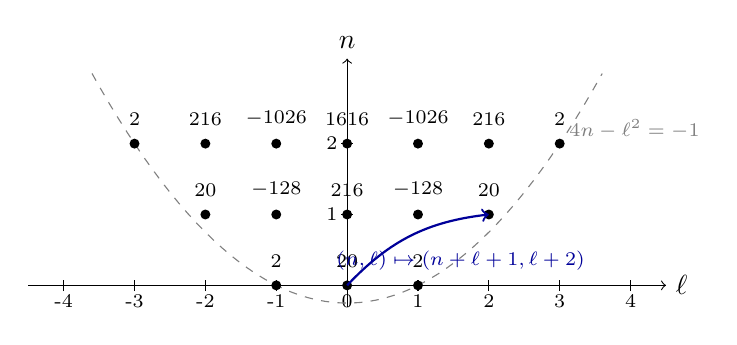
\begin{tikzpicture}[scale=0.9]
 \draw[->] (-4.5,0) -- (4.5,0) node[right] {$\ell$};
 \draw[->] (0,-0.3) -- (0,3.2) node[above] {$n$};
 \foreach \l in {-4,...,4} \draw (\l,-0.08) -- (\l,0.08) node[below=2pt,font=\scriptsize] {\l};
 \foreach \n in {1,2} \draw (-0.08,\n) -- (0.08,\n) node[left=2pt,font=\scriptsize] {\n};
 % parabola 4n - l^2 = -1, i.e. n = (l^2-1)/4
 \draw[dashed,gray] plot[domain=-3.6:3.6,samples=60] (\x,{(\x*\x-1)/4});
 \node[gray,font=\scriptsize,anchor=west] at (3.0,2.2) {$4n-\ell^2=-1$};
 % level 0
 \fill (-1,0) circle (2pt) node[above=3pt,font=\scriptsize] {2};
 \fill (0,0) circle (2pt) node[above=3pt,font=\scriptsize] {20};
 \fill (1,0) circle (2pt) node[above=3pt,font=\scriptsize] {2};
 % level 1
 \fill (-2,1) circle (2pt) node[above=3pt,font=\scriptsize] {20};
 \fill (-1,1) circle (2pt) node[above=3pt,font=\scriptsize] {$-128$};
 \fill (0,1) circle (2pt) node[above=3pt,font=\scriptsize] {216};
 \fill (1,1) circle (2pt) node[above=3pt,font=\scriptsize] {$-128$};
 \fill (2,1) circle (2pt) node[above=3pt,font=\scriptsize] {20};
 % level 2
 \fill (-3,2) circle (2pt) node[above=3pt,font=\scriptsize] {2};
 \fill (-2,2) circle (2pt) node[above=3pt,font=\scriptsize] {216};
 \fill (-1,2) circle (2pt) node[above=3pt,font=\scriptsize] {$-1026$};
 \fill (0,2) circle (2pt) node[above=3pt,font=\scriptsize] {1616};
 \fill (1,2) circle (2pt) node[above=3pt,font=\scriptsize] {$-1026$};
 \fill (2,2) circle (2pt) node[above=3pt,font=\scriptsize] {216};
 \fill (3,2) circle (2pt) node[above=3pt,font=\scriptsize] {2};
 % spectral flow arrow
 \draw[->,thick,blue!60!black] (0,0) to[bend left=20] (2,1);
 \node[blue!60!black,font=\scriptsize] at (1.6,0.35) {$(n,\ell)\mapsto(n+\ell+1,\ell+2)$};
\end{tikzpicture}
\caption{Support of the Fourier coefficients $c(n,\ell)$ of $\phi_{K3}$ in the
$(\ell,n)$ plane, with the values from \eqref{eq:ellgenus:expansion}. The coefficients are
constant along the parabolas $4n-\ell^2=\mathrm{const}$ and vanish below the dashed one.
The arrow is one unit of spectral flow \eqref{eq:ellgenus:jac2} with $\ell=1$, which maps
$c(0,0)=20$ to $c(1,2)=20$.}
\label{fig:ellgenus:support}
\end{figure}

\begin{pitfallbox}[Two normalizations of the same function]
$\phi_{K3}$ and $\phi_{0,1}=\tfrac12\phi_{K3}$ both appear in the literature. EOT use
$\phi_{K3}$ (Witten index $24$, coefficients $A_n=45,231,\dots$ with an explicit factor $2$ in
front of the massive characters); GHV use $\phi_{1A}=\phi_{0,1}$ (Witten index $12$) and
absorb the factor into their $A_n=90,462,\dots$ \source{GHV §3, ll.~578--580}. Neither is
wrong, but a table of ``the'' coefficients is meaningless without saying which normalization
it uses. This book follows the convention of \cref{ch:intro}: $A_n$ are EOT's numbers and the
multiplicities in the elliptic genus of K3 are $2A_n$.
\end{pitfallbox}

\section{\texorpdfstring{$N=4$}{N = 4} characters at \texorpdfstring{$c=6$}{c = 6}}\label{sec:ellgenus:chars}

The elliptic genus is a trace over a representation of the left-moving $N=4$ algebra
(tensored with right-moving ground states), so it can be written as a sum of the
\emph{characters} of the irreducible unitary representations,
\begin{equation}\label{eq:ellgenus:chardef}
 \mathrm{ch}^{\tilde R}_{h,\ell}(\tau,z)=\Tr_{\mathcal H_{h,\ell}}\,(-1)^F q^{L_0-c/24}y^{J_0},
\end{equation}
where the tilde on $R$ is the traditional reminder that $(-1)^F$ is inserted. At $c=6$
there are two kinds of representation in the Ramond sector.
\index{N=4 characters@$N=4$ characters}

\subsection{Massless (BPS) representations}

A representation whose highest-weight state has $h=\tfrac14=c/24$ is annihilated by $G_0$
and is called \emph{massless}\index{N=4 representations@$N=4$ representations!massless} or \emph{BPS}; the highest-weight state is a Ramond ground
state. Its $SU(2)$ spin is $\ell=0$ or $\ell=\tfrac12$. For $\ell=0$ the character is
\source{EOT §1, eqs.~(1.3)--(1.4), ll.~82--115}
\begin{align}
 \mathrm{ch}^{\tilde R}_{h=\frac14,\ell=0}(\tau,z)
   &=\frac{\vartheta_1(\tau,z)^2}{\eta(\tau)^3}\,\mu(\tau,z),\label{eq:ellgenus:ch0}\\
 \mu(\tau,z)&=\frac{-\ii\,\ee^{\pi\ii z}}{\vartheta_1(\tau,z)}
   \sum_{n\in\Z}\frac{(-1)^n q^{n(n+1)/2}\ee^{2\pi\ii nz}}{1-q^n\ee^{2\pi\ii z}}.
   \label{eq:ellgenus:mu}
\end{align}
The function $\mu$ is a \emph{Lerch sum}\index{Lerch sum} (or Appell--Lerch sum); it is not a Jacobi form
but a \emph{mock} modular object\index{mock modular form}, whose transformation law involves a non-holomorphic
correction \source{EOT §1, ll.~224--226}. This is the technical reason the massless
character, unlike the massive one below, has a complicated modular behaviour.

Let us extract the leading terms of \eqref{eq:ellgenus:ch0}, both to understand the
formula and because we will need them. From \eqref{eq:ellgenus:th1} and
\eqref{eq:ellgenus:eta},
\begin{equation}\label{eq:ellgenus:massive_core}
 \frac{\vartheta_1(\tau,z)^2}{\eta(\tau)^3}
 =q^{1/8}\Big[-(y-2+y^{-1})+q\,(2y^2-5y+6-5y^{-1}+2y^{-2})+O(q^2)\Big],
\end{equation}
the sign coming from $(-\ii)^2$ and the leading bracket from
$-y(1-y^{-1})^2=-(y-2+y^{-1})$. In the Lerch sum only the $n=0$ term, $1/(1-y)$, survives
at order $q^0$ (the term $n=-1$ has denominator $1-q^{-1}y$, which is $O(q)$ after
expansion), so with $\vartheta_1\approx-\ii q^{1/8}(y^{1/2}-y^{-1/2})$,
\begin{equation}\label{eq:ellgenus:mu_lead}
 \mu(\tau,z)=\frac{-\ii y^{1/2}}{-\ii q^{1/8}y^{1/2}(1-y^{-1})}\cdot\frac1{1-y}+O(q^{7/8})
 =-\frac{q^{-1/8}}{y-2+y^{-1}}+O(q^{7/8}).
\end{equation}
Multiplying, the poles cancel and
\begin{equation}\label{eq:ellgenus:ch0_exp}
 \mathrm{ch}^{\tilde R}_{\frac14,0}(\tau,z)
 =1+q\,(y^2-2y+2-2y^{-1}+y^{-2})+q^2\,(2y^2-6y+8-6y^{-1}+2y^{-2})+O(q^3),
\end{equation}
where the $q^1$ and $q^2$ terms are a symbolic check of this book. The leading $1$ is the
single ground state of $J_0=0$ (spin $\ell=0$), with $h-c/24=0$. The Witten index of the
representation is \source{EOT §1, eq.~(1.5), l.~114}
\begin{equation}\label{eq:ellgenus:ch0_index}
 \mathrm{ch}^{\tilde R}_{\frac14,0}(\tau,0)=1 ,
\end{equation}
as it must be: at $y=1$ every $q^n$ bracket in \eqref{eq:ellgenus:ch0_exp} vanishes
($1-2+2-2+1=0$, $2-6+8-6+2=0$), the excited states pairing off as in
\cref{sec:ellgenus:index}.

For $\ell=\tfrac12$ we use the relation \source{EOT §1, eq.~(1.10), ll.~160--169}
\begin{equation}\label{eq:ellgenus:split}
 q^{-1/8}\,\frac{\vartheta_1(\tau,z)^2}{\eta(\tau)^3}
 \;=\;2\,\mathrm{ch}^{\tilde R}_{\frac14,0}(\tau,z)+\mathrm{ch}^{\tilde R}_{\frac14,\frac12}(\tau,z),
\end{equation}
which expresses the fact that the massive representation of \cref{sec:ellgenus:massive}
becomes reducible at the unitarity bound $h=\tfrac14$ and splits into one $\ell=\tfrac12$
and two $\ell=0$ massless representations. Read as a definition of the $\ell=\tfrac12$
character, \eqref{eq:ellgenus:split} with \eqref{eq:ellgenus:massive_core} and
\eqref{eq:ellgenus:ch0_exp} gives
\begin{equation}\label{eq:ellgenus:chhalf_exp}
 \mathrm{ch}^{\tilde R}_{\frac14,\frac12}(\tau,z)=-(y+y^{-1})+q\,(-y+2-y^{-1})+O(q^2),
 \qquad \mathrm{ch}^{\tilde R}_{\frac14,\frac12}(\tau,0)=-2 .
\end{equation}
The ground states form an $SU(2)$ doublet of charges $J_0=\pm1$, i.e.\ $y^{\pm1}$, counted
with the sign $-1$: in the convention fixed by \eqref{eq:ellgenus:ch0}, where the $\ell=0$
ground state is bosonic, the doublet is fermionic. The Witten index $-2$ follows either from
the ground states or from \eqref{eq:ellgenus:split} at $z=0$, where the left side vanishes
because $\vartheta_1(\tau,0)=0$: $0=2\cdot1+\mathrm{ch}_{\frac14,\frac12}(\tau,0)$.

\subsection{Massive (non-BPS) representations}\label{sec:ellgenus:massive}

A representation with $h>\tfrac14$ is \emph{massive}\index{N=4 representations@$N=4$ representations!massive}. Its highest-weight state is not
annihilated by $G_0$, all four fermionic zero modes act freely on it, and the ground states
form the $2\times2=4$-dimensional representation of the zero-mode Clifford algebra: an
$SU(2)$ doublet and two singlets. The character is \source{EOT §1, eq.~(1.6), ll.~116--122}
\begin{equation}\label{eq:ellgenus:chmassive}
 \mathrm{ch}^{\tilde R}_{h,\ell=\frac12}(\tau,z)=q^{h-\frac38}\,\frac{\vartheta_1(\tau,z)^2}{\eta(\tau)^3}
 =q^{h-\frac14}\Big[-(y-2+y^{-1})+O(q)\Big].
\end{equation}
Check the bookkeeping of exponents: the trace starts at $q^{h-c/24}=q^{h-1/4}$, and
$\vartheta_1^2/\eta^3$ carries $q^{1/8}$, so the prefactor must be $q^{h-1/4-1/8}=q^{h-3/8}$.
The bracket is the four ground states: the two singlets with sign $+$ (the $2$) and the
doublet with sign $-$ (the $-y-y^{-1}$), the same sign pattern as the $\ell=\tfrac12$
massless representation. Every massive character vanishes at $z=0$ because
$\vartheta_1(\tau,0)=0$: a massive representation has Witten index zero. Only the massless
representations can contribute to the Euler number, which is why the coefficient of the
massless characters in the elliptic genus is topological, while the coefficients of the
massive ones can a priori depend on where we are in moduli space. (They do not, for K3, as we
now show; but the reason is the rigidity of $\phi_{K3}$, not the index argument.)

\begin{figure}[htbp]
\centering
\begin{tikzpicture}[scale=1, every node/.style={font=\scriptsize}]
 % massless l=0
 \draw[thick] (0,0) -- (1.2,0) node[right] {$J_0=0$, sign $+$};
 \node[anchor=east] at (-0.2,0) {$h=\tfrac14,\ \ell=0$:};
 \node at (0.6,-0.35) {index $+1$};
 % massless l=1/2
 \draw[thick] (4.6,0.25) -- (5.8,0.25) node[right] {$J_0=+1$, sign $-$};
 \draw[thick] (4.6,-0.25) -- (5.8,-0.25) node[right] {$J_0=-1$, sign $-$};
 \node[anchor=east] at (4.4,0) {$h=\tfrac14,\ \ell=\tfrac12$:};
 \node at (5.2,-0.65) {index $-2$};
 % massive
 \draw[thick] (0,-2.1) -- (1.2,-2.1) node[right] {$J_0=+1$, sign $-$};
 \draw[thick] (0,-1.7) -- (1.2,-1.7) node[right] {$J_0=0$ (two states), sign $+$};
 \draw[thick] (0,-1.5) -- (1.2,-1.5);
 \draw[thick] (0,-2.5) -- (1.2,-2.5) node[right] {$J_0=-1$, sign $-$};
 \node[anchor=east] at (-0.2,-2.0) {$h>\tfrac14$:};
 \node at (0.6,-2.9) {index $2-2=0$};
 \draw[->,gray] (4.6,-1.4) -- (4.6,-2.6);
 \node[gray,anchor=west] at (4.7,-2.0) {$h\to\tfrac14$: splits into $2\times(\ell=0)\ \oplus\ (\ell=\tfrac12)$};
\end{tikzpicture}
\caption{Ground states of the three kinds of Ramond representation of the $N=4$ algebra
at $c=6$, with their $J_0$ charge and the sign with which they enter the character
\eqref{eq:ellgenus:chardef}. The massive multiplet has four ground states and index zero; at
the unitarity bound it decomposes as in \eqref{eq:ellgenus:split}.}
\label{fig:ellgenus:multiplets}
\end{figure}

\section{Decomposing the elliptic genus}\label{sec:ellgenus:decomp}

\subsection{The decomposition and the function \texorpdfstring{$\Sigma$}{Sigma}}

Since every state of the K3 sigma model lies in some $N=4$ representation, and since the
elliptic genus is linear in the representation content, $\phi_{K3}$ must be a linear
combination of the characters of \cref{sec:ellgenus:chars} with integer coefficients. The
Witten index already fixes the massless part: writing
\begin{equation}\label{eq:ellgenus:decomp1}
 \phi_{K3}(\tau,z)=24\,\mathrm{ch}^{\tilde R}_{\frac14,0}(\tau,z)
 +\Sigma(\tau)\,\frac{\vartheta_1(\tau,z)^2}{\eta(\tau)^3}
\end{equation}
\source{EOT §1, eq.~(1.7), ll.~124--148} is consistent at $z=0$ because the second term
vanishes there and the first gives $24$. Everything not captured by $24$ copies of the
$\ell=0$ character has been put into a single function $\Sigma(\tau)$ multiplying the
massive character shape. That $\Sigma$ depends on $\tau$ only is a nontrivial statement:
$\phi_{K3}-24\,\mathrm{ch}_{\frac14,0}$ must be divisible by $\vartheta_1^2$ as a function
of $z$. Since both $\phi_{K3}$ and $\mathrm{ch}_{\frac14,0}$ are known in closed form, one can
solve for $\Sigma$, and EOT give the result \source{EOT §1, eqs.~(1.8)--(1.9), ll.~150--160}:
\begin{align}
 \Sigma(\tau)&=-8\Big[\mu\big(\tau;\tfrac12\big)+\mu\big(\tau;\tfrac{1+\tau}2\big)
   +\mu\big(\tau;\tfrac\tau2\big)\Big]\label{eq:ellgenus:Sigma}\\
 &=-2\,q^{-1/8}\Big(1-\sum_{n\ge1}A_nq^n\Big).\label{eq:ellgenus:Sigma_series}
\end{align}
The three arguments $\tfrac12,\tfrac{1+\tau}2,\tfrac\tau2$ are the three half-periods, the
same three that label $\vartheta_2,\vartheta_3,\vartheta_4$ in \eqref{eq:ellgenus:ZK3}.
Equation \eqref{eq:ellgenus:Sigma_series} \emph{defines} the coefficients $A_n$\index{A_n@$A_n$ (EOT coefficients)}. We checked
\eqref{eq:ellgenus:Sigma}--\eqref{eq:ellgenus:Sigma_series} numerically to forty digits at two
values of $\tau$ with the nine coefficients of \eqref{eq:ellgenus:An_table} below, and checked
that $(\phi_{K3}-24\,\mathrm{ch}_{\frac14,0})\eta^3/\vartheta_1^2$ is independent of $z$; these
are symbolic checks, not Tier~A.

The polar term $-2q^{-1/8}$ in \eqref{eq:ellgenus:Sigma_series} is not a massive
representation (it would have $h-\tfrac14=-\tfrac18<0$). It is removed by the splitting
relation \eqref{eq:ellgenus:split}: $-2q^{-1/8}\vartheta_1^2/\eta^3=-4\,\mathrm{ch}_{\frac14,0}
-2\,\mathrm{ch}_{\frac14,\frac12}$, and the final form of the decomposition is
\source{EOT §1, eq.~(1.11), ll.~169--195}
\begin{equation}\label{eq:ellgenus:decomp2}
 \boxed{\;\phi_{K3}(\tau,z)=20\,\mathrm{ch}^{\tilde R}_{\frac14,0}(\tau,z)
 -2\,\mathrm{ch}^{\tilde R}_{\frac14,\frac12}(\tau,z)
 +2\sum_{n\ge1}A_n\,q^{\,n-\frac18}\,\frac{\vartheta_1(\tau,z)^2}{\eta(\tau)^3}\;}
\end{equation}
The third term is $2A_n$ copies of the massive character with $h=n+\tfrac14$, by
\eqref{eq:ellgenus:chmassive}. Check the Witten index once more: $20\cdot1-2\cdot(-2)+0=24$.
Check the $q^0$ term with \eqref{eq:ellgenus:ch0_exp} and \eqref{eq:ellgenus:chhalf_exp}:
$20\cdot1-2\cdot(-y-y^{-1})=20+2y+2y^{-1}$, which is \eqref{eq:ellgenus:q0}. The twenty
$\ell=0$ representations are the twenty $(1,1)$-classes; the $-2$ copies of the
$\ell=\tfrac12$ representation, entering with a minus sign because its ground states are
fermionic in our convention, supply the four charged ground states $H^{0,0},H^{2,0},H^{0,2},
H^{2,2}$.

\begin{pitfallbox}[A negative multiplicity is not a negative number of states]
The coefficient $-2$ in \eqref{eq:ellgenus:decomp2} does not mean that the K3 sigma model
contains ``minus two'' representations. The multiplicity of the $\ell=\tfrac12$
representation in the full Hilbert space, tensored with right-moving ground states, is a
non-negative integer; the sign is produced by the right-moving factor $(-1)^{\bar F}$ in
\eqref{eq:ellgenus:def}, which weights right-moving Ramond ground states by $\pm1$. The
elliptic genus counts left-moving representations \emph{with a sign} that depends on the
right-moving partner. Similarly $2A_n$ is a signed count; that it is positive for all $n$ is
the content of the positivity conjecture recalled in \cref{sec:ellgenus:An}.
\end{pitfallbox}

\subsection{Worked example: \texorpdfstring{$A_1=45$}{A1 = 45} and \texorpdfstring{$A_2=231$}{A2 = 231} by hand}\label{sec:ellgenus:worked2}

The decomposition \eqref{eq:ellgenus:decomp2} can be solved for the $A_n$ order by order
in $q$, using only the expansions already written down. At order $q^1$ the left side is the
$q^1$ bracket of \eqref{eq:ellgenus:expansion}; on the right we need the $q^1$ terms of the
two massless characters and the $q^0$ term of $q^{-1/8}\vartheta_1^2/\eta^3$ from
\eqref{eq:ellgenus:massive_core}:
\begin{align*}
 20y^2-128y+216-128y^{-1}+20y^{-2}
 ={}&20\,(y^2-2y+2-2y^{-1}+y^{-2})-2\,(-y+2-y^{-1})\\
 &+2A_1\,\big(-y+2-y^{-1}\big).
\end{align*}
Compare coefficients. Of $y^2$: $20=20$, no information (the massive ground states carry
$|J_0|\le1$). Of $y^1$: $-128=-40+2-2A_1$, so $2A_1=90$ and $A_1=45$. Of $y^0$:
$216=40-4+4A_1$, so $A_1=45$ again, a consistency check. At order $q^2$ one needs the $q^2$
terms of the massless characters, the $q^1$ term of the massive core (multiplied by $2A_1$)
and its $q^0$ term multiplied by $2A_2$; the $y^0$ coefficient gives
$1616=20\cdot8-2\cdot4+90\cdot6+4A_2$, i.e.\ $4A_2=924$ and $A_2=231$. Both values agree with
\source{EOT §1, eq.~(1.12), ll.~197--209}. The student is asked to redo the $y^{\pm1}$ and
$y^{\pm2}$ coefficients at order $q^2$ in \cref{exe:ellgenus:A2}.

\subsection{The coefficients \texorpdfstring{$A_n$}{An}}\label{sec:ellgenus:An}

EOT tabulate \source{EOT §1, eq.~(1.12), ll.~197--209}
\begin{equation}\label{eq:ellgenus:An_table}
\begin{array}{c|ccccccccc}
 n   & 1 & 2 & 3 & 4 & 5 & 6 & 7 & 8 & 9\\ \hline
 A_n & 45 & 231 & 770 & 2277 & 5796 & 13915 & 30843 & 65550 & 132825
\end{array}
\end{equation}
and recall the conjecture that all $A_n$ are positive integers \source{EOT §1, l.~210};
integrality is clear from \eqref{eq:ellgenus:decomp2}, positivity is not. Support for
positivity comes from the asymptotic formula obtained by Eguchi and Hikami by a
Rademacher-type expansion \source{EOT §1, eq.~(1.13), ll.~211--223}, which we write as
\begin{equation}\label{eq:ellgenus:asymp}
 A_n\;\approx\;\frac{2}{\sqrt{8n-1}}\,\exp\!\Big(\frac{\pi}{2}\sqrt{8n-1}\Big)
 \;=\;\frac{2}{\sqrt{8n-1}}\,\exp\!\Big(2\pi\sqrt{\tfrac12\big(n-\tfrac18\big)}\Big).
\end{equation}
The text extraction of EOT's equation garbles the prefactor, so we fixed it by a numerical
check: the ratio of $A_n$ to $\ee^{\pi\sqrt{8n-1}/2}/\sqrt{8n-1}$ is
\begin{equation*}
 1.87,\quad 2.04,\quad 1.98,\quad 2.02,\quad 1.99,\quad 2.01,\quad 1.996,\quad 2.002,\quad 1.998
 \qquad(n=1,\dots,9),
\end{equation*}
converging to $2$ (a symbolic check of this book). The exponent has the Cardy form
\begin{equation*}
 \exp\Big(2\pi\sqrt{\tfrac{c_{\rm eff}}{6}\big(n-\tfrac18\big)}\Big)
 \qquad\text{with}\qquad c_{\rm eff}=3,
\end{equation*}
not $6$: the growth of the coefficients of a modular or mock modular form is set by its most
polar term, and the polar term of $\Sigma$ is $q^{-1/8}=q^{-c_{\rm eff}/24}$ (standard; not
checked against a source in this book's library). As \source{EOT §1, ll.~222--224} remark, the formula is a good estimate even at small
$n$, which is why it supports positivity.

\begin{example}[The growth of $A_n$]
For $n=5$, $\sqrt{8n-1}=\sqrt{39}=6.245$, the exponent is $\pi\cdot6.245/2=9.809$,
$\ee^{9.809}=1.82\times10^4$, and $2/6.245=0.320$, giving $A_5\approx5.83\times10^3$ against
the exact $5796$, an error of $0.7\%$. For $n=1$ the same recipe gives $48$ against $45$.
\end{example}

\subsection{The observation}

Now compare \eqref{eq:ellgenus:An_table} with the list of dimensions of the irreducible
representations of the Mathieu group $\Mtf$\index{Mathieu group $\Mtf$!irreducible dimensions} (\cref{ch:m24}): $1$, $23$, $45$, $45$, $231$,
$231$, $252$, $253$, $483$, $770$, $770$, $990$, $990$, $1035$, $1035$, $1035$, $1265$,
$1771$, $2024$, $2277$, $3312$, $3520$, $5313$, $5796$, $5544$, $10395$
\source{EOT App.~A, eq.~(A.3), ll.~345--349}. The first five $A_n$ are on the list, and the next two
are sums of entries \source{EOT §1, eqs.~(1.14)--(1.15), ll.~228--237}:
\begin{equation}\label{eq:ellgenus:A6A7}
 A_6=13915=3520+10395,\qquad A_7=30843=10395+5796+5544+5313+2024+1771 .
\end{equation}
For $n\ge8$ decompositions exist but are no longer unique \source{EOT §1, ll.~238--239}.
That is the whole of the observation, and the numerical part of it is exactly what the Lean
library checks (\cref{sec:ellgenus:lean}). What it might \emph{mean} is the subject of
\cref{ch:moonshine}: the natural conjecture is that the space of states of the K3 sigma
model at each massive level carries an action of $\Mtf$ of which $2A_n$ is the graded
dimension, in the same way that the coefficients $196884,\dots$ of the modular function
$J(q)$ are graded dimensions of a representation of the Monster group
\source{EOT §1, eq.~(1.16), ll.~240--255}. The mystery, in EOT's words, is that no K3
surface has $\Mtf$ as a symmetry group: the finite groups of symplectic automorphisms of K3
surfaces enumerated by Mukai are all proper subgroups of $\Mtf$ (\cref{ch:m24}), and the
question is whether the elliptic genus, which is constant over the whole moduli space, sees
a symmetry that no single point of moduli space possesses \source{EOT §1, ll.~268--275}.

\begin{historybox}
The observation was made, according to the authors' acknowledgment, at the Aspen Center for
Physics during the workshop ``Unity of String Theory'' \source{EOT, ll.~318--319}. EOT's
first version of the paper contained a different decomposition of $A_7$; the one in
\eqref{eq:ellgenus:A6A7} is the corrected version, chosen to be consistent with the
twisted elliptic genera computed in later work \source{EOT §1, footnote~1, ll.~257--259}.
GHV, whose normalization gives $2A_7=61686$, note that even the corrected decomposition is
consistent with, but not uniquely fixed by, their twining characters
\source{GHV §3, eq.~(3.4), ll.~575--583}.
\end{historybox}

\subsection{The factor two: \texorpdfstring{$2A_n$}{2 An} and real representations}\label{sec:ellgenus:2An}

The factor $2$ in front of the massive characters in \eqref{eq:ellgenus:decomp2} is
physical. GHV absorb it and write \source{GHV §3, eqs.~(3.1)--(3.3), ll.~500--577}
\begin{equation}\label{eq:ellgenus:ghv}
 24=23+1,\qquad -A_0^{\rm GHV}=2=1+1,\qquad A_1^{\rm GHV}=90=45+45,\quad
 A_2^{\rm GHV}=462=231+231,\quad\dots
\end{equation}
for the rescaled genus $\phi_{1A}=\tfrac12\phi_{K3}$. In their normalization every
multiplicity is the dimension of a \emph{real} representation of $\Mtf$: $45+\overline{45}$,
$231+\overline{231}$, and so on, where $\overline{45}$ is the complex conjugate of the
$45$-dimensional representation (the two entries $45,45$ in the list above). This is
natural, because a graded vector space that is the ``space of states'' of a real field theory
should carry a real representation. In EOT's normalization the same statement reads: the
multiplicity of the massive representation at level $n$ in the K3 elliptic genus is $2A_n$,
with $A_n$ the dimension of one of the two conjugate irreducible representations. The
massless part reads, in GHV's form, $24=23+1$ for the $\ell=0$ representations (the
$23$-dimensional permutation representation of $\Mtf$ on $24$ points, minus the trivial
one) and $-2=-(1+1)$ for the $\ell=\tfrac12$ representation. This book's convention
(\cref{ch:intro}) is EOT's: $A_n$ denotes $45,231,770,\dots$, and the multiplicities are
$2A_n$.

\subsection{The NS-sector function}\label{sec:ellgenus:ns}

Monstrous moonshine is formulated for the partition function of a bosonic theory, a
function of $\tau$ alone. To make the analogy tight, GHV apply spectral flow by
$\eta=\tfrac12$ to the left-movers and remove the $(-1)^F$, which shifts $z$ by
$\tfrac\tau2+\tfrac12$ \source{GHV §2, eqs.~(2.7)--(2.8), ll.~168--187}:
\begin{equation}\label{eq:ellgenus:nsdef}
 \chi(\tau,z)=\exp\!\Big[2\pi\ii m\Big(\frac\tau4+z+\frac12\Big)\Big]\,
 \phi\Big(\tau,z+\frac\tau2+\frac12\Big).
\end{equation}
For K3 with $m=1$ and $\phi=\phi_{1A}$, set $z=0$. The substitution sends
$y\mapsto\ee^{2\pi\ii(\tau/2+1/2)}=-q^{1/2}$ and the prefactor is $-q^{1/4}$, so from
\eqref{eq:ellgenus:expansion} divided by $2$,
\begin{align}
 \chi_{1A}(\tau)&=-q^{1/4}\Big[(-q^{1/2}+10-q^{-1/2})+q\,(10q+64q^{1/2}+108+64q^{-1/2}+10q^{-1})
   +\dots\Big]\notag\\
 &=q^{-1/4}\big(1-20\,q^{1/2}-62\,q-216\,q^{3/2}-\dots\big),\label{eq:ellgenus:ns}
\end{align}
which agrees with \source{GHV §2, eq.~(2.11), ll.~228--254} in the two terms they display
(they also give the closed form $(2\vartheta_4(\tau)/\vartheta_2(\tau))^2-(2\vartheta_2(\tau)/
\vartheta_4(\tau))^2$, which we checked numerically). The leading power $q^{-1/4}=q^{-c/24}$
is the NS vacuum, exactly as $q^{-1}=q^{-24/24}$ is the vacuum of the Monster theory in
$J(q)$, and the function transforms under the subgroup of $\SLZ$ generated by $T^2$ and $S$
\source{GHV §2, eqs.~(2.9)--(2.10), ll.~188--227}. It is this function, and its ``twined''
versions with a group element inserted in the trace, that \cref{ch:moonshine} studies.

\section{What the machine has checked}\label{sec:ellgenus:lean}

Nothing in the analytic part of this chapter is formalized: theta functions, Jacobi forms,
the $N=4$ algebra and its characters are all Tier~L, pinned to EOT and GHV above. What the
Lean library checks is the arithmetic at the two ends of the story: the central charge $6$
and the chiral-primary count $2$ as fixed rational and natural numbers, and the assertion
that the tabulated $A_n$ are dimensions, or sums of dimensions, of irreducible
representations of $\Mtf$. The three files are
\begin{itemize}[leftmargin=1.5em,itemsep=0pt]
\item \lean{StringTheoryFormalization/Frontier/CentralCharge.lean},
\item \lean{StringTheoryFormalization/Frontier/ChiralPrimaries.lean},
\item \lean{DualScaleStream2/Moonshine/EOT.lean}.
\end{itemize}
All audited theorems depend only on the axioms \lean{propext}, \lean{Classical.choice} and
\lean{Quot.sound}.

\begin{leanbox}[In Lean: the coefficients $A_1,\dots,A_9$ and $\Mtf$]
\begin{leancode}
/-- EOT eq. (1.12): `A₁, …, A₉`. -/
def eotA : Fin 9 → ℕ := ![45, 231, 770, 2277, 5796, 13915, 30843, 65550, 132825]

/-- `A₁ … A₅` are each the dimension of an irreducible representation
    of `M₂₄`. -/
theorem first_five_are_irreps :
    ∀ n : Fin 5, ∃ i : Fin 26,
      M24RepDim i = eotA (Fin.castLE (by norm_num) n) := by ...

/-- EOT eq. (1.14): `A₆ = 3520 + 10395`, both irreducible dimensions
    (indices 21, 25). -/
theorem A6_decomposition :
    eotA 5 = M24RepDim 21 + M24RepDim 25 := rfl

/-- EOT eq. (1.15): `A₇ = 10395 + 5796 + 5544 + 5313 + 2024 + 1771`. -/
theorem A7_decomposition :
    eotA 6 = M24RepDim 25 + M24RepDim 23 + M24RepDim 24 + M24RepDim 22 +
      M24RepDim 18 + M24RepDim 17 := rfl

/-- `A₆` is *not* a single irreducible dimension (so a decomposition is
    genuinely needed). -/
theorem A6_not_irrep : ∀ i : Fin 26, M24RepDim i ≠ eotA 5 := by ...
\end{leancode}
\emph{Reading.} \lean{eotA} is the table \eqref{eq:ellgenus:An_table}, typed in by hand
from EOT; Lean indexes from $0$, so \lean{eotA 5} is $A_6$. \lean{M24RepDim} is the
$26$-entry list of irreducible dimensions of $\Mtf$ from another library
(\lean{StringTheoryFormalization/StringDynamics/MathieuM24.lean}, discussed in
\cref{ch:m24}), in the increasing order of EOT's eq.~(A.3). \lean{first\_five\_are\_irreps}
says: for each of the five indices $n=0,\dots,4$ there exists an index $i$ into the list with
\lean{M24RepDim i = eotA n}. It is an existence statement with explicit witnesses
($i=2,4,9,19,23$); it does not say that $45$ is the dimension of a \emph{unique} irreducible
representation (it is not: the list contains $45$ twice), and it says nothing about $\Mtf$
acting on anything. \lean{A6\_decomposition} and \lean{A7\_decomposition} are the two
equations \eqref{eq:ellgenus:A6A7}, with each summand named by its position in the list.
\lean{A6\_not\_irrep} says that no entry of the list equals $13915$, so that the
decomposition of $A_6$ into two summands is not a disguised triviality. None of these
theorems mentions the elliptic genus, a character, or a group: they are statements about two
finite lists of natural numbers. \emph{Proof idea.} \lean{first\_five\_are\_irreps} is a
case split on \lean{n : Fin 5}, each case closed by exhibiting the witness and \lean{rfl};
the two decompositions are \lean{rfl} because both sides reduce to numerals; the
non-membership is a case split over all $26$ indices closed by \lean{decide}.
\end{leanbox}

\begin{leanbox}[In Lean: $c=6$ and the two chiral primaries]
\begin{leancode}
def centralChargeBoson : ℚ := 1
def centralChargeFermion : ℚ := 1/2
def centralChargeK3 : ℚ :=
  4 * centralChargeBoson + 4 * centralChargeFermion
theorem central_charge_k3_eq_six : centralChargeK3 = 6 := by ...

structure N2State where
  confWeight : ℚ
  u1Charge : ℚ
def bpsBound (s : N2State) : Prop :=
  s.confWeight ≥ |s.u1Charge| / 2
def isChiralPrimary (s : N2State) : Prop :=
  0 ≤ s.u1Charge ∧ s.confWeight = s.u1Charge / 2
theorem chiral_primary_saturates_bps (s : N2State) (h : isChiralPrimary s) :
    bpsBound s := by ...

def K3ChiralPrimaryCount : Fin 3 → ℕ
  | ⟨0, _⟩ => 1  -- H^{0,0} = ℂ (vacuum)
  | ⟨1, _⟩ => 0  -- H^{1,0} = 0 (K3 has no holomorphic 1-forms)
  | ⟨2, _⟩ => 1  -- H^{2,0} = ℂ (holomorphic 2-form Ω)
theorem k3_chiral_primary_total :
    (∑ i : Fin 3, K3ChiralPrimaryCount i) = 2 := by ...
\end{leancode}
\emph{Reading.} These are arithmetic shadows of \cref{sec:ellgenus:n4}.
\lean{central\_charge\_k3\_eq\_six} says $4\cdot1+4\cdot\tfrac12=6$ in $\Q$, with the two
free-field values entered as constants; no stress tensor or operator product expansion is
involved, and the theorem would be equally true if K3 did not exist. \lean{N2State} is a
pair of rationals $(h,q)$ with no positivity constraint on $h$. \lean{bpsBound} is
\eqref{eq:ellgenus:bps} and \lean{isChiralPrimary} is ``$q\ge0$ and $h=q/2$'';
\lean{chiral\_primary\_saturates\_bps} proves the one direction ``chiral primary
$\Rightarrow$ bound holds'', which is immediate because $|q|=q$ for $q\ge0$. Nothing about
the $N=2$ algebra, its representations, or which states of a given theory are chiral
primaries is formalized. \lean{K3ChiralPrimaryCount} is the table $(1,0,1)$ typed in by
hand, not derived from the Hodge numbers of \cref{ch:k3}, and \lean{k3\_chiral\_primary\_total}
sums it to $2$. \emph{Proof idea.} \lean{norm\_num} on the constants; \lean{simp} with
\lean{abs\_of\_nonneg}; and \lean{Fin.sum\_univ\_three} followed by \lean{simp}.
\end{leanbox}

\begin{pitfallbox}[Names that promise more than the statement delivers]
The same file contains three declarations whose names must not be read as theorems about
physics. \lean{virasoro\_ope\_central\_term} takes points $z,w\in\C$ with $z\ne w$ as
arguments and never uses them: it proves \lean{centralChargeK3 / 2 = 3}, a numeral identity,
not a statement about the $T(z)T(w)$ operator product.
\lean{virasoro\_algebra\_commutator} takes a function \lean{L : ℤ → ℤ} that does not appear
in its conclusion, the polynomial identity $\tfrac c{12}(m^3-m)=\tfrac{c\,m(m^2-1)}{12}$, true
for every rational $c$. \lean{central\_charge\_from\_worldsheet\_action} is
$\exists c,\ c=\lean{centralChargeK3}\wedge c=6$, witnessed by $6$. And in the chiral-primary
file, \lean{chiral\_primary\_ring\_associativity} takes three chiral primaries as hypotheses
and concludes \lean{True}: no chiral ring, no structure constants, no associativity is
defined, let alone proved. The docstrings in the files say all this explicitly; a reader of
the catalogue who sees only the names would be misled. The rule of \cref{ch:intro} applies:
read the statement, not the name.
\end{pitfallbox}

\begin{leanbox}[Related declarations in other libraries]
The older \lean{DualScaleM24Formalization} library records the same numerology in GHV's
normalization: \lean{SocrateAI.Moonshine.dimA1} is the constant $90$ and
\lean{dimA1\_decomposition} proves \lean{dimA1 = 45 + 45}, with companions for $462$ and
$1540$; these are decidable equalities between numerals. The Euler number $24$ that fixes
the elliptic genus is \lean{SocrateAI.Moonshine.k3\_euler\_eq\_24}, the alternating sum of
the Betti numbers $(1,0,22,0,1)$ entered as constants (see \cref{ch:tadpole}).
\end{leanbox}

\begin{center}
\begin{tabular}{@{}p{0.55\textwidth}cp{0.3\textwidth}@{}}
\toprule
Claim & Tier & Where \\
\midrule
Witten index counts $E=0$ states with sign and is deformation invariant & \TL & derived in
 \cref{sec:ellgenus:index}; standard \\
Elliptic genus is a weak Jacobi form of weight $0$, index $c/6$ & \TL & GHV §2 \\
$J^{\rm weak}_{0,1}$ is one-dimensional; $\phi_{K3}=2\phi_{0,1}$ & \TL & EOT §1 \\
$\phi_{K3}=8\sum_{i=2,3,4}(\vartheta_i(z)/\vartheta_i(0))^2$, $\phi_{K3}(\tau,0)=24$ & \TL &
 EOT eq.~(1.2); expansion \eqref{eq:ellgenus:expansion} symbolically checked \\
$N=4$ characters \eqref{eq:ellgenus:ch0}, \eqref{eq:ellgenus:chmassive}, splitting
 \eqref{eq:ellgenus:split} & \TL & EOT eqs.~(1.3)--(1.6), (1.10) \\
Decomposition \eqref{eq:ellgenus:decomp2}, table \eqref{eq:ellgenus:An_table} & \TL & EOT
 eqs.~(1.11)--(1.12); $A_1,A_2$ re-derived by hand, $\Sigma$ checked numerically \\
$A_n>0$ for all $n$ & \TC & conjecture recalled in EOT, l.~210 \\
$c_{K3}=4\cdot1+4\cdot\frac12=6$ as rational arithmetic & \TA & \lean{central\_charge\_k3\_eq\_six} \\
$1+0+1=2$ chiral primaries as a hand-entered table & \TA & \lean{k3\_chiral\_primary\_total} \\
$A_1,\dots,A_5$ occur in the list of $\Mtf$ irreducible dimensions & \TA &
 \lean{first\_five\_are\_irreps} \\
$A_6$, $A_7$ equal EOT's sums of list entries; $A_6$ is not an entry & \TA &
 \lean{A6\_decomposition}, \lean{A7\_decomposition}, \lean{A6\_not\_irrep} \\
The list \lean{M24RepDim} is the list of irreducible dimensions of $\Mtf$ & \TL & EOT
 eq.~(A.3); see \cref{ch:m24} \\
The K3 elliptic genus carries an $\Mtf$ action & \TL/\TC & \cref{ch:moonshine} \\
\bottomrule
\end{tabular}
\end{center}

\begin{summarybox}
\begin{itemize}[leftmargin=1.2em,itemsep=1pt]
\item The Witten index $\Tr(-1)^F\ee^{-\beta H}$ counts zero-energy states with sign; excited
 states cancel in boson--fermion pairs, so the index is an integer and a deformation
 invariant.
\item The elliptic genus \eqref{eq:ellgenus:def} applies the cancellation to the
 right-movers only and keeps $q^{L_0-c/24}$ and $y^{J_0}$ for the left-movers. It is
 holomorphic in $\tau$, and a weak Jacobi form of weight $0$ and index $m=c/6$. Its
 specializations give $\chi$ ($z=0$), the signature up to sign ($z=\tfrac12$, $q^0$ term) and
 the $\chi_y$ genus ($q^0$ term).
\item The K3 sigma model has $c=6$, $N=4$ superconformal symmetry, two chiral primaries, and
 index $m=1$. The space of weak Jacobi forms of weight $0$ and index $1$ is one-dimensional,
 so $\phi_{K3}$ is fixed by $\chi(K3)=24$; explicitly, \eqref{eq:ellgenus:ZK3}, with the
 expansion \eqref{eq:ellgenus:expansion} whose coefficients depend only on $4n-\ell^2$.
\item Ramond representations of the $N=4$ algebra at $c=6$: massless with $\ell=0$ (index
 $1$), massless with $\ell=\tfrac12$ (index $-2$), massive with $h>\tfrac14$ (index $0$,
 character $q^{h-3/8}\vartheta_1^2/\eta^3$). At $h=\tfrac14$ the massive character splits as
 $2\,\mathrm{ch}_{\frac14,0}+\mathrm{ch}_{\frac14,\frac12}$.
\item $\phi_{K3}=20\,\mathrm{ch}_{\frac14,0}-2\,\mathrm{ch}_{\frac14,\frac12}
 +2\sum_{n\ge1}A_nq^{n-1/8}\vartheta_1^2/\eta^3$ with $A_n=45,231,770,2277,5796,\dots$;
 multiplicities are $2A_n$ (EOT convention, used in this book). The first five $A_n$ are
 dimensions of irreducible representations of $\Mtf$, $A_6$ and $A_7$ are sums of such.
\item Lean checks the arithmetic ends only: $c=6$, the chiral-primary count $2$, and the
 membership of $A_1,\dots,A_5$ (and the decompositions of $A_6,A_7$) in the list of
 $\Mtf$ dimensions. Everything analytic is Tier~L.
\end{itemize}
\end{summarybox}

\section*{Exercises}
\addcontentsline{toc}{section}{Exercises}

\begin{exercise}[$\star$]
A supersymmetric quantum mechanics has supercharge $Q$ with $Q^2=H$ and a Hilbert space
spanned by states of energies $0,0,0,3,3,7,7,7,7$ with $(-1)^F=(+,+,-,+,-,+,-,+,-)$. Compute
$\Tr(-1)^F\ee^{-\beta H}$ and verify that it is independent of $\beta$. Which states could be
lifted from $E=0$ by a small deformation, and which could not?
\end{exercise}

\begin{exercise}[$\star$]
Using the Hodge diamond of K3 ($h^{0,0}=h^{2,0}=h^{0,2}=h^{2,2}=1$, $h^{1,1}=20$), compute
the $\chi_y$ genus $\sum_{p,q}(-1)^{p+q}h^{p,q}y^{p-1}$ and check it against
\eqref{eq:ellgenus:q0}. Then compute the same quantity for $T^4$ ($h^{p,q}=\binom2p\binom2q$)
and explain why the elliptic genus of $T^4$ vanishes identically.
\end{exercise}

\begin{exercise}[$\star\star$]
Verify the three expansions of the theta ratios used in \cref{sec:ellgenus:worked1} from the
products \eqref{eq:ellgenus:th2}--\eqref{eq:ellgenus:th4}, then square and add to obtain the
$q^1$ term of \eqref{eq:ellgenus:expansion}. Where do the half-integer powers of $q$ cancel,
and why must they?
\end{exercise}

\begin{exercise}[$\star\star$]\label{exe:ellgenus:A2}
Extend the computation of \cref{sec:ellgenus:worked2} to the $y^{\pm1}$ and $y^{\pm2}$
coefficients at order $q^2$ (the $q^2$ terms of the massless characters are in
\eqref{eq:ellgenus:ch0_exp} and \eqref{eq:ellgenus:chhalf_exp}; you will need the $q^2$ term
of $\vartheta_1^2/\eta^3$, which is $q^{1/8}(-y^3+6y^2-15y+20-15y^{-1}+6y^{-2}-y^{-3})$).
Show that all of them give $A_2=231$. Why does the $y^{\pm3}$ coefficient give no
information about $A_2$?
\end{exercise}

\begin{exercise}[$\star\star$]
Show from \eqref{eq:ellgenus:jac2} with $\ell=1$ that the coefficients of a weak Jacobi
form of index $m$ satisfy $c(n,\ell)=c(n+\ell+m,\ell+2m)$, and deduce that $c(n,\ell)$
depends only on $4mn-\ell^2$ and on $\ell\bmod2m$. Check the statement on
\cref{tab:ellgenus:coeffs}. Then use the spectral flow \eqref{eq:ellgenus:flow} with
$\eta=1$ to give the same identity a physical meaning.
\end{exercise}

\begin{exercise}[$\star\star$]
Evaluate the asymptotic formula \eqref{eq:ellgenus:asymp} for $n=10$ and $n=20$, and
compare with the values $A_{10}=260568$ and $A_{20}=63\,447\,087$, which are not in EOT's
table \eqref{eq:ellgenus:An_table} but were extracted for this book from
\eqref{eq:ellgenus:Sigma} numerically (a symbolic check, not a sourced datum; the same
computation reproduces $A_1,\dots,A_9$). How does the relative error decrease with $n$?
\end{exercise}

\begin{exercise}[$\star\star\star$]
Write the massive character \eqref{eq:ellgenus:chmassive} as $q^{h-1/4}$ times a
$y$-Laurent polynomial at each level and interpret the level-one term
$2y^2-5y+6-5y^{-1}+2y^{-2}$ of \eqref{eq:ellgenus:massive_core} as the action of the modes
$L_{-1}$, $J^a_{-1}$ ($a=1,2,3$) and $G^{\pm}_{-1}$, $G^{\pm\prime}_{-1}$ of the $N=4$ algebra
on the four ground states. (Count: which combinations of one bosonic or one fermionic mode
on each ground state give the stated charges and signs?)
\end{exercise}

\begin{exercise}[$\star\star$, Lean]
State and prove in Lean, in the style of \lean{A6\_decomposition}, that $A_8=65550$ can be
written as a sum of entries of \lean{M24RepDim} (find a decomposition by hand first; EOT
remark that it is not unique). Then state the analogue of \lean{A6\_not\_irrep} for $A_8$.
\end{exercise}

\begin{exercise}[$\star\star\star$, Lean]
Replace the hand-entered table \lean{K3ChiralPrimaryCount} by a definition that reads the
counts $h^{p,0}$ from a Hodge-number table \lean{h : Fin 3 → Fin 3 → ℕ} (as in
\lean{eulerFromHodge} of \cref{ch:tadpole}), and re-prove
\lean{k3\_chiral\_primary\_total} for the K3 table. What extra hypothesis would you need for
the statement ``the number of chiral primaries equals $\sum_ph^{p,0}$'' to be a theorem
about a conformal field theory rather than about a table?
\end{exercise}

\section*{Further reading}
\addcontentsline{toc}{section}{Further reading}
\begin{itemize}[leftmargin=1.5em]
\item The definition of the elliptic genus for hyperk\"ahler targets, the theta-function
 formula for K3, the $N=4$ characters, the decomposition, the table of $A_n$, the
 asymptotic formula, and the observation about $\Mtf$ with its comparison to monstrous
 moonshine: \source{EOT §1, ll.~39--308}. The dimensions of the irreducible representations
 of $\Mtf$: \source{EOT App.~A, eq.~(A.3), ll.~345--349}.
\item Jacobi-form properties of elliptic genera, the $q$-expansion of $\phi_{K3}$, spectral
 flow, and the NS-sector function $\chi(\tau)$ with its modular behaviour under
 $\langle T^2,S\rangle$: \source{GHV §2, ll.~104--294}. The decomposition in GHV's
 normalization with real representations, $24=23+1$, $90=45+45$, \dots:
 \source{GHV §3, eqs.~(3.1)--(3.4), ll.~500--583}. Theta-function conventions:
 \source{GHV App.~A, eq.~(A.1), ll.~1453--1490}.
\item The K3 moduli space over which the elliptic genus is constant: \cref{ch:stringsk3};
 the orbifold point $T^4/\Z_2$: \cref{ch:kummer}; the group $\Mtf$ and its representations:
 \cref{ch:m24}; what is now known about the action of $\Mtf$ on the space of states:
 \cref{ch:moonshine}.
\end{itemize}
